\documentclass[border=3pt]{standalone}
\usepackage{tikz}
\usetikzlibrary{arrows.meta,automata,positioning}
\begin{document}
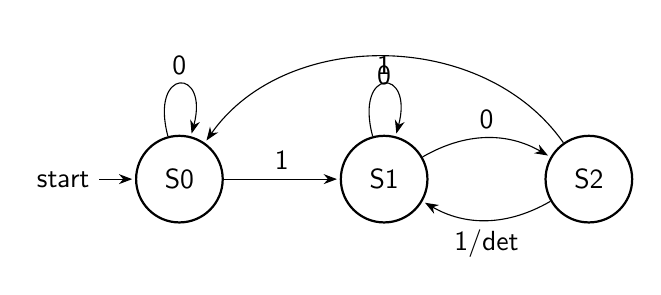
\begin{tikzpicture}[font=\sffamily,
    >=Stealth, shorten >=1pt, node distance=26mm, on grid, auto,
    every state/.style={thick, minimum size=11mm}]
  % A "101" sequence detector (Mealy-ish state names)
  \node[state, initial] (s0) {S0};
  \node[state, right=of s0] (s1) {S1};
  \node[state, right=of s1] (s2) {S2};
  \path[->]
    (s0) edge[loop above] node{0} ()
    (s0) edge node{1} (s1)
    (s1) edge[bend left] node{0} (s2)
    (s1) edge[loop above] node{1} ()
    (s2) edge[bend left] node[below]{1/det} (s1)
    (s2) edge[bend right=55] node[below]{0} (s0);
\end{tikzpicture}
\end{document}
